\chapter{System Design}

\section{Introduction}
In this chapter, we move from the analysis phase to a concrete technical solution. 
Based on the identified system requirements, we present the system design through UML diagrams and database modeling.

The main objective is to define the system architecture and its underlying data structure.

\section{Class Diagram}
A class diagram is a UML diagram that describes the static structure of a system by representing its classes, 
their attributes, methods, and the relationships between them \cite{booch2005uml}. 
It provides a global view of the system architecture.

\begin{figure}[H]
	\centering
	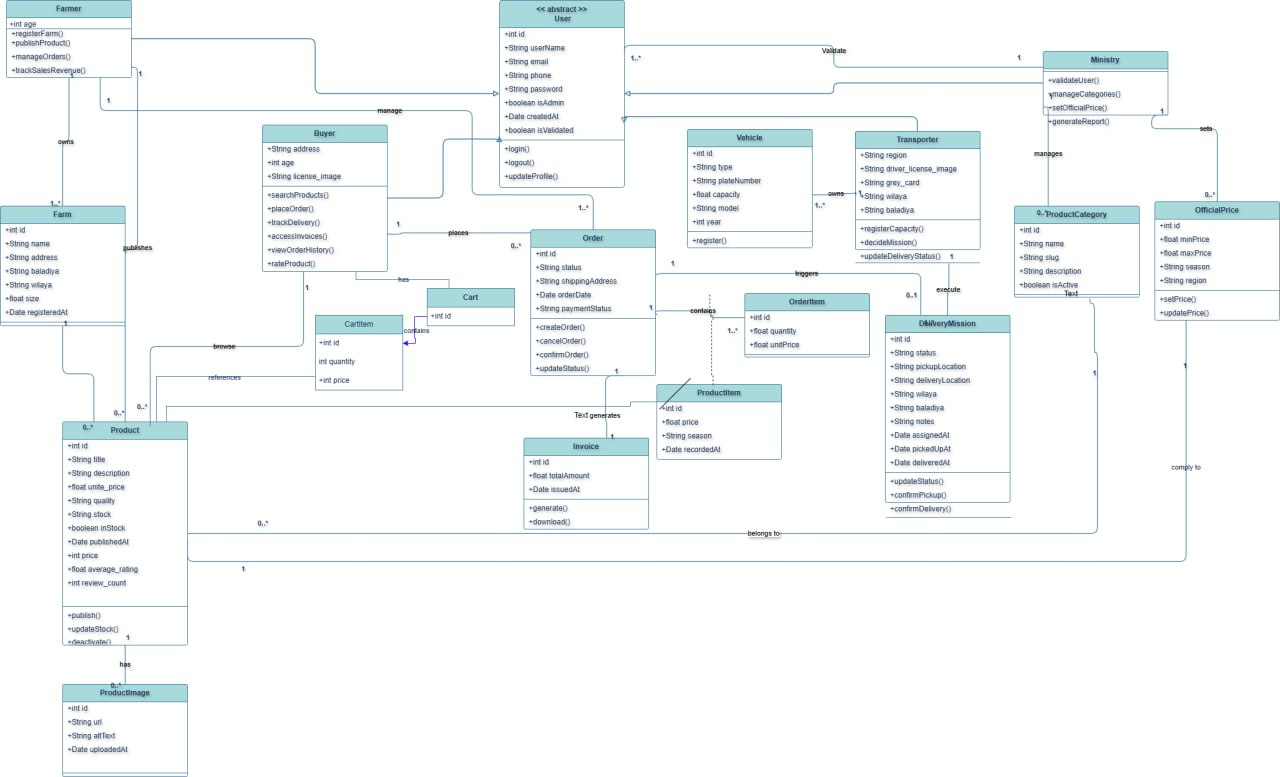
\includegraphics[width=0.9\linewidth]{images/diagrammes/diagramme_classe}
	\caption{Class Diagram of the System}
\end{figure}

\section{Database Design}

\subsection{Object-Relational Mapping Rules}
The transformation from the object-oriented model to the relational model is based on the following rules \cite{elmasri2016database,fowler2002patterns}:

\begin{itemize}
	\item Each class is mapped to a table
	\item Each attribute is mapped to a column
	\item The identifier becomes the primary key
	\item Associations are translated into foreign keys
	\item Many-to-many relationships are implemented using junction tables
\end{itemize}

These rules are directly applied based on the class diagram.

\subsection{Relational Schema}
The relational schema of the system is defined as follows:

\begin{itemize}
	\item \textbf{Farmer} (\underline{id}, userName, email, phone, createdAt, isValidated)
	\item \textbf{Buyer} (\underline{id}, userName, email, phone, createdAt, address)
	\item \textbf{Transporter} (\underline{id}, userName, email, phone, createdAt, region)
	\item \textbf{Ministry} (\underline{id}, userName, email, phone, createdAt)
	
	\item \textbf{Farm} (\underline{id}, name, location, gpsCoordinates, wilaya, registeredAt, \#farmerId)
	
	\item \textbf{ProductCategory} (\underline{id}, name, slug, description, isActive)
	
	\item \textbf{OfficialPrice} (\underline{id}, minPrice, maxPrice, season, region, \#ministryId, \#categoryId)
	
	\item \textbf{PriceHistory} (\underline{id}, price, season, setAt, \#officialPriceId)
	
	\item \textbf{Product} (\underline{id}, name, unit, quality, stock, inStock, publishedAt, price, \#farmId, \#categoryId)
	
	\item \textbf{ProductImage} (\underline{id}, url, altText, isCover, uploadedAt, \#productId)
	
	\item \textbf{ProductHistory} (\underline{id}, price, season, recordedAt, reason, \#productId)
	
	\item \textbf{Order} (\underline{id}, status, shippingAddress, orderDate, paymentStatus, \#buyerId)
	
	\item \textbf{OrderItem} (\underline{id}, quantity, unitPrice, \#orderId, \#productId)
	
	\item \textbf{Invoice} (\underline{id}, totalAmount, issuedAt, \#orderId)
	
	\item \textbf{Vehicle} (\underline{id}, type, plateNumber, capacity, carteGrise, \#transporterId)
	
	\item \textbf{DeliveryMission} (\underline{id}, status, pickupLocation, deliveryLocation, assignedAt, pickedUpAt, deliveredAt, \#orderId, \#transporterId, \#vehicleId)
\end{itemize}

\begin{figure}[H]
	\centering
	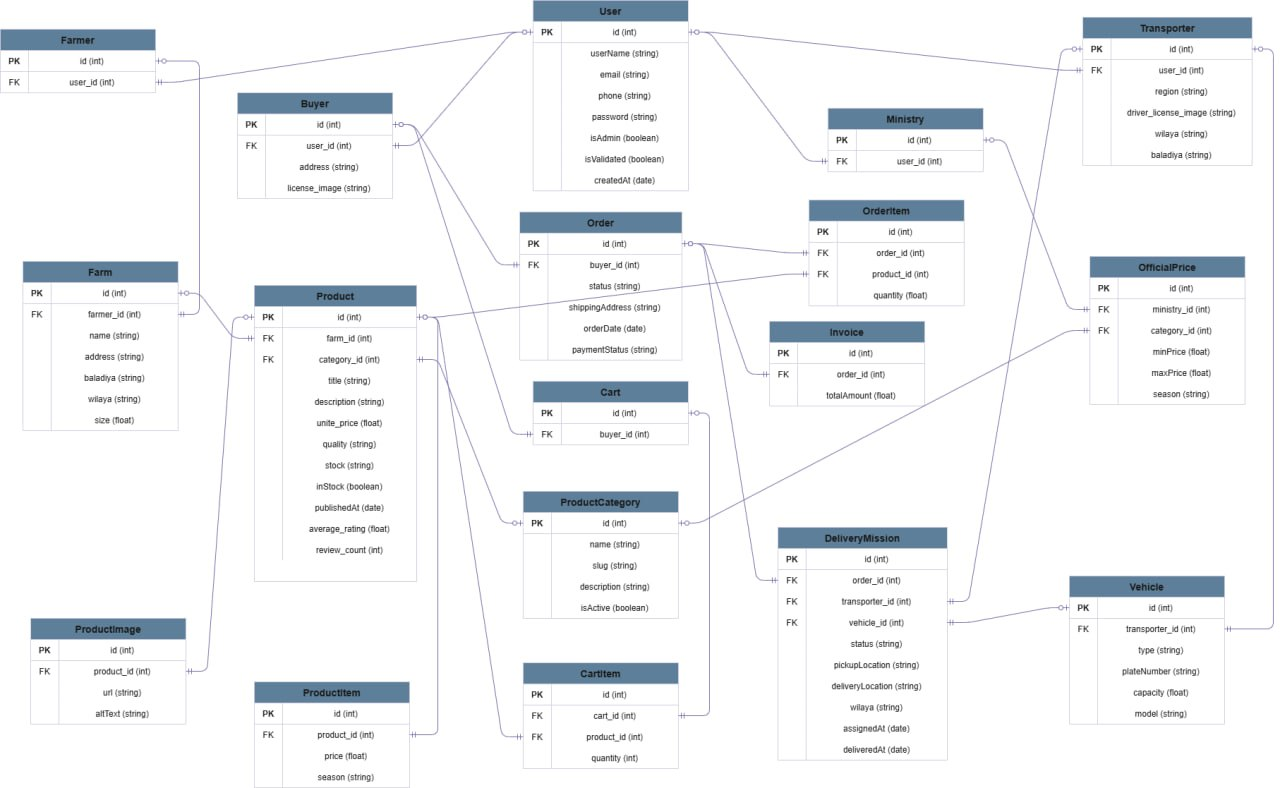
\includegraphics[width=1.1\linewidth]{images/diagrammes/schema_relationnel}
	\caption{Schéma relationnel}
\end{figure}
